\documentclass[answers]{exam}

\usepackage[utf8]{inputenc}
\usepackage[english]{babel}
\usepackage{amsmath}
\usepackage{tikz}
\usepackage{booktabs}
\usepackage{units}

\usetikzlibrary{arrows,decorations.pathmorphing,backgrounds,positioning}
\newcommand{\degree}{^\circ}

\CorrectChoiceEmphasis{\bfseries \color{red}}

\begin{document}
\lhead{\bfseries\large PHY102M\\Robbie Rosati}
\rhead{\bfseries\large Lab Final\\November 30th, 2015}
    
Your name:\enspace\makebox[2.5in]{\hrulefill} Version: Key %VERSION_LETTER
\begin{center}
    \fbox{\fbox{\parbox{5.7in}{\centering
        Fill out your name and your UT ID on your scantron.
        Calculators and your cheat sheet (one page) allowed.
        Mark each answer on your scantron and your paper. Pencil only.
        Do not repeat the contents of this test to anyone. Return both to desk.
        Common constants are on the back.
    }}}
\end{center}

\begin{questions}

\question When we graph $V$ vs. $U$, which variable is dependent, and which is independent?
%NO RANDOMIZE
\begin{choices}
\choice Both are dependent.
\choice Both are independent.
\choice $V$ is independent, $U$ is dependent.
\CorrectChoice $U$ is independent, $V$ is dependent.
\choice None of the above
\end{choices}

\question If I asked you to graph $V$ vs $U$, and gave you the relation $3 V = \frac{q}{4 e} U + f$, what would you expect the slope to be?
\begin{choices}
\CorrectChoice $\frac{q}{12 e}$
\choice $\frac{\frac{4}{3} e}{q}$
\choice $3$
\choice $f$
\choice $1/f$
\end{choices}

\question If I shoot a cannonball straight up at $v_y = 1,000 \textrm{ m/s}$, how long will it take to return to the ground (rounded to the nearest second)? Neglect air resistance, and assume the cannonball remains low enough that $g$ is constant.
\begin{choices}
\choice The cannonball never hits the ground.
\CorrectChoice $\unit[204]{s}$
\choice $\unit[102]{s}$
\choice $\unit[20]{s}$
\choice $\unit[156]{s}$
\end{choices}

\question You measure the length of two objects as $30 \pm 0.5 \textrm{ cm}$ and $27 \pm 0.3 \textrm{ cm}$. What is the \textbf{difference} of these values, with uncertainty?
\begin{choices}
\choice $\unit[3.0 \pm 0.2]{cm}$
\CorrectChoice $\unit[3.0 \pm 0.8]{cm}$ 
\choice $\unit[57  \pm 0.8]{cm}$
\choice $\unit[3.0 \pm 0.083]{cm}$
\choice $\unit[3.0 \pm 0.0]{cm}$
\end{choices}

\question Spiders sometimes hang from their webs to catch insects. You are a spider, and to catch a tasty bug you need to be perfectly balanced. If three forces on you are $F_1 = \unit[3\boldsymbol{\hat{x}} - 2\boldsymbol{\hat{y}} + 1\boldsymbol{\hat{z}}]{N}$, $F_2 = \unit[2\boldsymbol{\hat{x}} + 2\boldsymbol{\hat{y}} - 2\boldsymbol{\hat{z}}]{N}$, and $F_3 = \unit[-0.5\boldsymbol{\hat{x}} - 5\boldsymbol{\hat{y}} + 3\boldsymbol{\hat{z}}]{N}$, what fourth force would you need to balance yourself?
\begin{choices}
\choice $\unit[4.5\boldsymbol{\hat{x}} - 5\boldsymbol{\hat{y}} + 2\boldsymbol{\hat{z}}]{N}$
\CorrectChoice $\unit[-4.5\boldsymbol{\hat{x}} + 5\boldsymbol{\hat{y}} - 2\boldsymbol{\hat{z}}]{N}$ 
\choice You are already balanced
\choice $\unit[-4.5\boldsymbol{\hat{x}} + 5\boldsymbol{\hat{y}} + 2\boldsymbol{\hat{z}}]{N}$
\choice $\unit[1.5\boldsymbol{\hat{x}} + 3\boldsymbol{\hat{y}} - 2\boldsymbol{\hat{z}}]{N}$
\end{choices}

\question In lab 3, we had a cart roll down an inclined plane, with friction. If the cart rolled downhill, which way did the force of friction act on the cart?
\begin{choices}
\choice Downhill
\CorrectChoice Uphill 
\choice Down (into the surface of the ramp)
\choice Up (out of the surface of the ramp)
\choice Left or right
\end{choices}

\question Recall that, in lab 3, we had a cart roll down an inclined plane, with friction, and with a weighted hangar pulling the cart. If some Martians tried this experiment on Mars ($g_\textrm{MARS} \approx \frac{1}{3} g_\textrm{EARTH}$), their cart's measured acceleration would be a fraction of the acceleration we measured in RLM.

If we measured the cart's acceleration to be $a = \unit[3.0]{m/s^2}$, a Martian with an identical experimental setup would measure
%NO RANDOMIZE
\begin{choices}
\CorrectChoice $\unit[1.0]{m/s^2}$ 
\choice $\unit[3.0]{m/s^2}$
\choice $\unit[6.0]{m/s^2}$
\choice $\unit[9.8]{m/s^2}$
\choice None of the above
\end{choices}

\question A pendulum of length $\unit[1500]{cm}$ is held at a $\unit[60]{\degree}$ angle from the vertical. What will be the bob's maximum velocity after it is released?
%NO RANDOMIZE
\begin{choices}
\CorrectChoice $\unit[12.1]{m/s}$ 
\choice $\unit[1210]{m/s}$
\choice $\unit[16.0]{m/s}$
\choice $\unit[6.28]{m/s}$
\choice None of the above
\end{choices}

\question If we place a block on top of a frictionless ramp at angle $30\degree$, $\unit[2]{m}$ above the ground, how fast is the block moving when it reaches the ground?

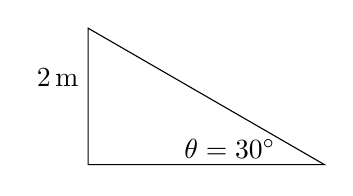
\begin{tikzpicture}[scale=1]
\draw (0,0) -- (-3,0) -- (-3,1.732) -- cycle;
\node at (-1.2,.2) {$\theta = 30\degree$};
\node at (-3,0.866) [above left] {\unit[2]{m}};
\end{tikzpicture}

\begin{choices}
\choice $\unit[19.6]{m/s}$
\choice $\unit[39.2]{m/s}$
\choice $\unit[4.43]{m/s}$
\CorrectChoice $\unit[6.26]{m/s}$ 
\choice Need mass to calculate
\end{choices}

\question The International Table Tennis Federation limits the coefficient of restitution ($C_R = \frac{v_{2f} - v_{1f}}{v_{1i}-v_{2i}}$) for balls to the range $0.89$ to $0.92$. If you were cheating and used a ball with a $C_R$ of $1$, what would happen?
%NO RANDOMIZE
\begin{choices}
\choice The ball would be more likely to spin.
\choice The ball would be less bouncy, but still work.
\choice The ball would collide perfectly inelastically with the table, and stick to it.
\choice The ball would jump from the table more quickly than it was hit toward the table, as if an explosion had increased its kinetic energy.
\CorrectChoice None of the above 
\end{choices}

\question You and another person are rushing to class in opposite directions at the same speed. You collide perfectly elastically. If the total kinetic energy of both people was initially $\unit[300]{kJ}$, what would be the kinetic energy of both people after the collision?
\begin{choices}
\CorrectChoice $\unit[300]{kJ}$ 
\choice $\unit[150]{kJ}$
\choice $\unit[200]{kJ}$
\choice $\unit[100]{kJ}$
\choice $\unit[0]{kJ}$
\end{choices}

\question If you replace the back wheel of a bike with a larger wheel, is the bike easier or harder to pedal (all else being equal)?
\begin{choices}
\CorrectChoice Harder 
\choice Easier
\choice No change
\choice Need more information
\end{choices}

\question If you apply a force of $F = \unit{50}{N}$ to a disk with a $\unit[2]{m}$ radius and a $\unit[68]{kg}$ mass using a pulley with a radius of $\unit[30]{cm}$, what is your expected angular acceleration?

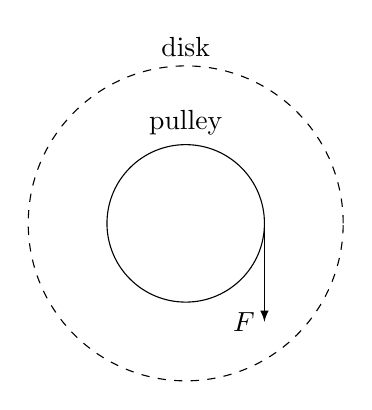
\begin{tikzpicture}[scale=.5]
\draw (0,0) circle (2);
\node at (0,2) [above] {pulley};
\draw [-latex] (2,0) -- (2,-2.5) node [left] {$F$};
\draw [dashed] (0,0) circle (4);
\node at (0,4) [above] {disk};
\end{tikzpicture}

\begin{choices}
\CorrectChoice $\unitfrac[0.110]{rad}{s^2}$ 
\choice $\unitfrac[0.735]{rad}{s^2}$
\choice $\unitfrac[4.90]{rad}{s^2}$
\choice $\unitfrac[32.7]{rad}{s^2}$
\choice $\unitfrac[15.0]{rad}{s^2}$
\end{choices}

\question What's the angular momentum of a thin bar, mass $\unit[5.0]{kg}$ and length $\unit[1.0]{m}$, spinning around its center at $\unitfrac[1.0]{rad}{s}$?
\begin{choices}
\CorrectChoice $\unit[0.42]{kg m^2/s}$ 
\choice $\unit[0.42]{kg/s}$
\choice $\unit[0.42]{g m^2/s}$
\choice $\unit[1.67]{kg m^2 s}$
\choice $\unit[1.67]{g m^2 s}$
\end{choices}

\question The buoyant force on a floating object is equal to
%NO RANDOMIZE
\begin{choices}
\choice its weight
\choice the weight of the water it displaces
\choice more than its weight
\CorrectChoice both choice A and B 
\choice both B and C
\end{choices}

\question What field of physics have we been studying in this class?
\begin{choices}
\CorrectChoice Classical Mechanics 
\choice Electrodynamics
\choice Quantum Mechanics
\choice Statistical Mechanics
\end{choices}

\question A sea urchin with a volume of $\unit[50]{mL}$ displaces how much water, when completely immersed?
\begin{choices}
\choice Need mass of sea urchin
\CorrectChoice $\unit[50]{mL}$ 
\choice $\unit[100]{mL}$
\choice Need to know shape of sea urchin
\choice No water is displaced
\end{choices}

\question A mass on a spring is harmonically oscillating at $\unit[2]{Hz}$, and travels up to $\unit[50]{cm}$ from the equilibrium point of the spring. What is the maximum acceleration experienced by the mass?
\begin{choices}
\choice Need more information
\choice $\unit[200]{m/s^2}$
\CorrectChoice $\unit[79]{m/s^2}$ 
\choice $\unit[2.0]{m/s^2}$
\choice $\unit[6.3]{m/s^2}$
\end{choices}

\question You're Jill the Pendulum Maker, and you're making a pendulum that will be much longer than the distance it moves back and forth. If you want to calculate its period, what approximation can you make?
\begin{choices}
\choice The angle from the vertical, $\theta$, can be considered $\approx 90\degree$. $\sin{\theta} \approx 1$
\CorrectChoice The angle from the vertical, $\theta$, can be considered very small. $\sin{\theta} \approx \theta$ 
\choice The pendulum's mass can be set to zero.
\choice The pendulum's motion can be ignored. Period of the pendulum $T \rightarrow \infty$.
\choice Miley Cyrus can ride your pendulum like a wrecking ball.
\end{choices}

\question In lab 10, we made standing waves on a string. We found up to $8$ harmonics. How far apart were these harmonics spaced, in multiples of the fundamental frequency?
\begin{choices}
\CorrectChoice $1$ 
\choice $0.5$
\choice $2$
\choice $8$
\choice $1.5$
\end{choices}

\question If we had vibrated a rectangular plate instead of a square plate in lab 10, we would expect the sand to form different patterns. If we gradually increased the frequency, starting from $\unit[0]{Hz}$, we would expect the first node to appear along which direction of the plate?
\begin{choices}
\choice Along the shorter direction, or the sand will form a line parallel with the long edge of the plate.
\CorrectChoice Along the longer direction, or the sand will form a line parallel with the short edge of the plate.
\choice The first node will appear along both directions.
\choice The first mode won't exist.
\choice The sand will form a line along the diagonal of the plate.
\end{choices}



\question Spaceman Spiff pours $\unit[3]{L}$ of liquid nitrogen (at its boiling point) into $\unit[5]{L}$ of $\unit[25\degree]{C}$ water. What is the water's final temperature, and did it freeze?
\begin{choices}
\CorrectChoice $\unit[0\degree]{C}$, partially frozen 
\choice $\unit[0\degree]{C}$, completely frozen
\choice $\unit[-3.8\degree]{C}$, completely frozen
\choice $\unit[3.8\degree]{C}$ liquid
\choice $\unit[-196\degree]{C}$, completely frozen
\end{choices}

\question How many times more energy does it take to turn water into steam than to heat it from $\unit[0\degree]{C}$ to $\unit[100\degree]{C}$? In other words, what is $E_\textrm{complete boiling}/E_\textrm{heating}$?
\begin{choices}
\choice 0.185
\choice 6.26
\choice 0.798
\CorrectChoice 5.40
\choice 0.480
\end{choices}

\end{questions}

\pagebreak

\begin{center}
\begin{tabular}{@{}rl@{}}
    \textbf{Quantity}            & \textbf{Value}                 \\ \midrule
    Standard acceleration of gravity & $\unitfrac[9.80665]{m}{s^2}$ \\
    Speed of light                   & $\unitfrac[299792458]{m}{s}$ \\
    Speed of sound standard temperature and pressure & \unitfrac[343.2]{m}{s}\\
    Density of water          & $\unitfrac[1.00]{g}{cm^3}$ \\
    Density of aluminum       & $\unitfrac[2.70]{g}{cm^3}$ \\
	Density of steel          & $\unitfrac[7.83]{g}{cm^3}$ \\
	Density of brass          & $\unitfrac[8.44]{g}{cm^3}$ \\
	Density of copper         & $\unitfrac[8.96]{g}{cm^3}$ \\
    Density of liquid nitrogen & $\unitfrac[0.808]{g}{cm^3}$ \\
	Specific heat of water                        & $\unitfrac[4186]{J}{kgK}$ \\
    Specific heat of ice ($\unit[-10\degree]{C}$) & $\unitfrac[2000]{J}{kgK}$ \\
    Specific heat of aluminum                     & $\unitfrac[900]{J}{kgK}$ \\
    Specific heat of copper                       & $\unitfrac[386]{J}{kgK}$ \\
    Latent heat of vaporization, water     & $\unitfrac[2.260\times10^6]{J}{kg}$\\
    Latent heat of vaporization, nitrogen  & $\unitfrac[2.01\times10^5]{J}{kg}$\\    Latent heat of vaporization, helium    & $\unitfrac[2.1\times10^4]{J}{kg}$\\
    Latent heat of sublimation, water    & $\unitfrac[3.34\times10^5]{J}{kg}$\\
    Temperature of boiling liquid nitrogen & $\unit[-195.79\degree \pm 0.01\degree]{C}$ \\
    Temperature of boiling liquid helium   & $\unit[-268.9\degree]{C}$ \\
    Temperature of boiling water           & $\unit[100\degree]{C}$ \\
    Temperature of melting ice             & $\unit[0\degree]{C}$   \\
\end{tabular}
\tikzset{inmm/.style={x=1mm,y=1mm, baseline=-0.5ex,
          show background rectangle,
          inner frame sep=2pt,
          background rectangle/.style={
          draw=none
        }}}

\begin{tabular}{@{}crl@{}}
     & \textbf{Situation}            & \textbf{Inertia}                 \\      \midrule
    \tikz[inmm]{
        \draw (0,0) circle (5);
        \draw [fill=black] (0,0) circle (1);}
    & Disk/Cylinder, around center, radius $R$ & $I=\frac{1}{2} MR^2$ \\
    \tikz[inmm]{
        \draw (0,0) circle (5);
        \draw (0,0) circle (4);
        \draw [fill=black] (0,0) circle (1);}
    & Ring, around center, radii from $R_1$ to $R_2$ & $I=\frac{1}{2} M \left(  R_1^2 + R_2^2 \right)$ \\
    \tikz[inmm]{
        \path [use as bounding box] (0,0) circle (5);
        \draw (-5,-1) rectangle (5,1);
        \draw (-4.5,0) [fill=black] circle (1);}
    & Thin bar, around edge, length $L$ & $I=\frac{1}{3} M L^2$ \\
    \tikz[inmm]{
        \path [use as bounding box] (0,0) circle (5);
        \draw (-5,-1) rectangle (5,1);
        \draw (0,0) [fill=black] circle (1);}
    & Thin bar, around center, length $L$ & $I=\frac{1}{12} M L^2$ \\
    \tikz[inmm]{
        \path [use as bounding box] (0,0) circle (5);
        \draw (-5,-4) rectangle (5,4);
        \draw (0,0) [fill=black] circle (1);}
    & Rectangle, around center, $W$ by $L$ & $I=\frac{1}{12} M \left( L^2 +     W^2 \right)$ \\
\end{tabular}

\end{center}

\end{document}
